\documentclass{beamer}
\usepackage[english]{babel}
\usetheme{default}

\author{{\scriptsize T. Fossati, P. Giacomin, S. Loreto, M. Rossini}}
\title{CoAP Options for Sleepy Nodes}
\institute{{\large IETF 83, Paris}}
\date{}

\begin{document}

\begin{frame}[plain]
 \titlepage
\end{frame}

%%
%% Intro
%% 
\begin{frame}{Intro}

\begin{itemize}
 \item Two I-Ds for three Options :-)
 \item Extend Proxies capabilities to help Sleepy nodes participate in CoAP networks
 \item Each Option employs a different technique to solve specific (orthogonal) issues that surface when the \emph{always on} postulate is negated
\end{itemize}

\end{frame}

\begin{frame}{Options}

\begin{itemize}
 \item \textbf{Sleepy.}  Allow end to end communication between two sleepy nodes using the Proxy as a \emph{store and forward} agent;
 \vspace{.3cm}
 \item \textbf{Publish.}  Allow generic CoAP nodes to interact with a resource hosted at a sleepy node by (temporarily) delegating the resource to a Proxy;
 \vspace{.3cm}
 \item \textbf{Monitor.}  Make Observe bootstrap possible in case two sleepy nodes are involved.
\end{itemize}

\end{frame}


%%
%% Sleepy option 
%%
\begin{frame}{Sleepy  \hspace{6cm} {\tiny \texttt{draft-giacomin-core-sleepy-option-00}}}

\begin{itemize}
 \item Use Proxy as \emph{store and forward} agent for Sleepy to Sleepy messaging
 \item TODO
\end{itemize}

\end{frame}

%%
%% Publish option 
%%
\begin{frame}{Publish \hspace{5cm} {\tiny \texttt{draft-fossati-core-publish-monitor-options-01}}}

\begin{itemize}
 \item Sleepy node asks Proxy to serve its resource(s)
 \item Handle the whole delegation life-time: \mbox{\small{Publish $\rightarrow$ Update $\rightarrow$ ... $\rightarrow$ Update $\rightarrow$ (implicit) Remove}}
 \item Sleepy node may specify allowed methods %%(support writable resources, default GET only)
\end{itemize}

\end{frame}

%%
%% Publish (pic: publish resource)
%%
\begin{frame}{(1) Publish resource}
 \begin{center}
  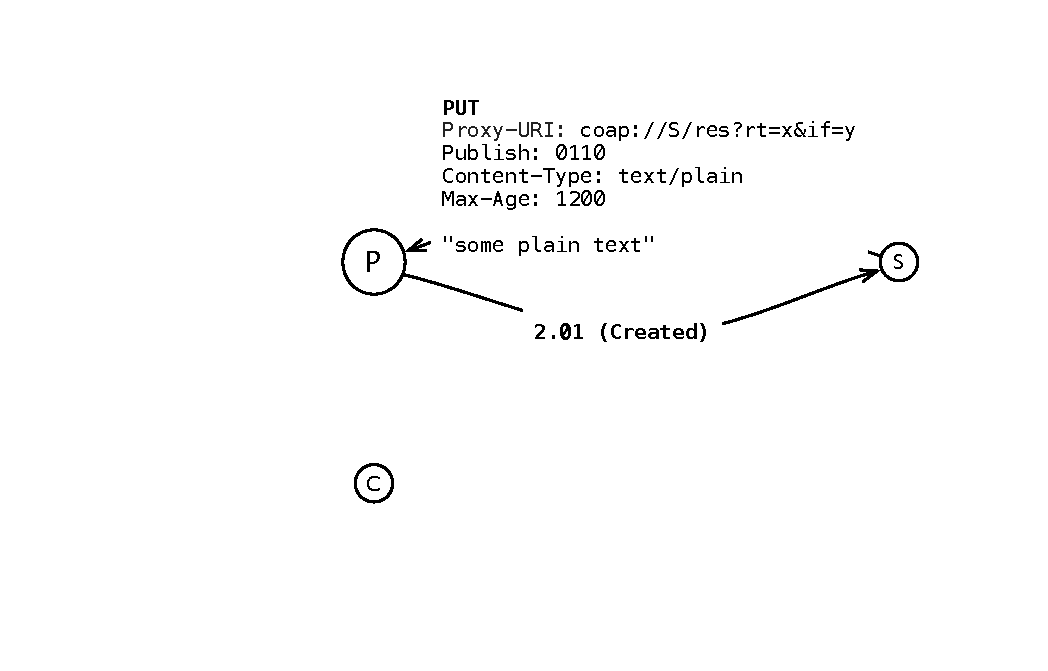
\includegraphics[width=\textwidth]{../../share/images/publish0.pdf}
 \end{center}
\end{frame}

%%
%% Publish (pic: retrieve published resource)
%%
\begin{frame}{(2) Act on published resource}
 \begin{center}
  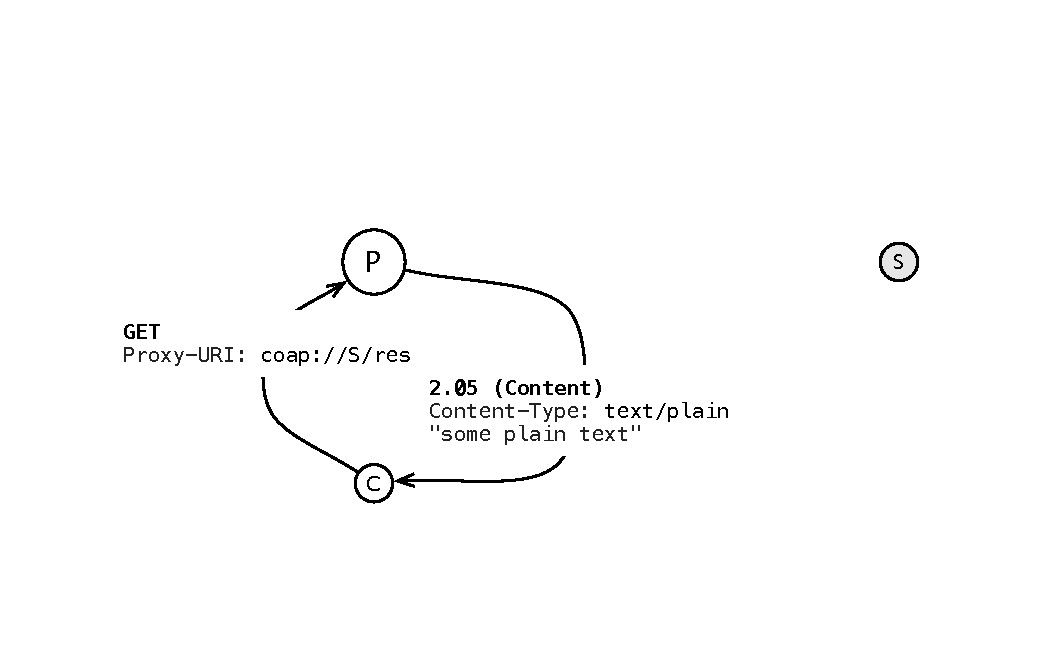
\includegraphics[width=\textwidth]{../../share/images/publish1.pdf}
 \end{center}
\end{frame}

%%
%% Publish (pic: update published resource)
%%
\begin{frame}{(3) Update published resource}
 \begin{center}
  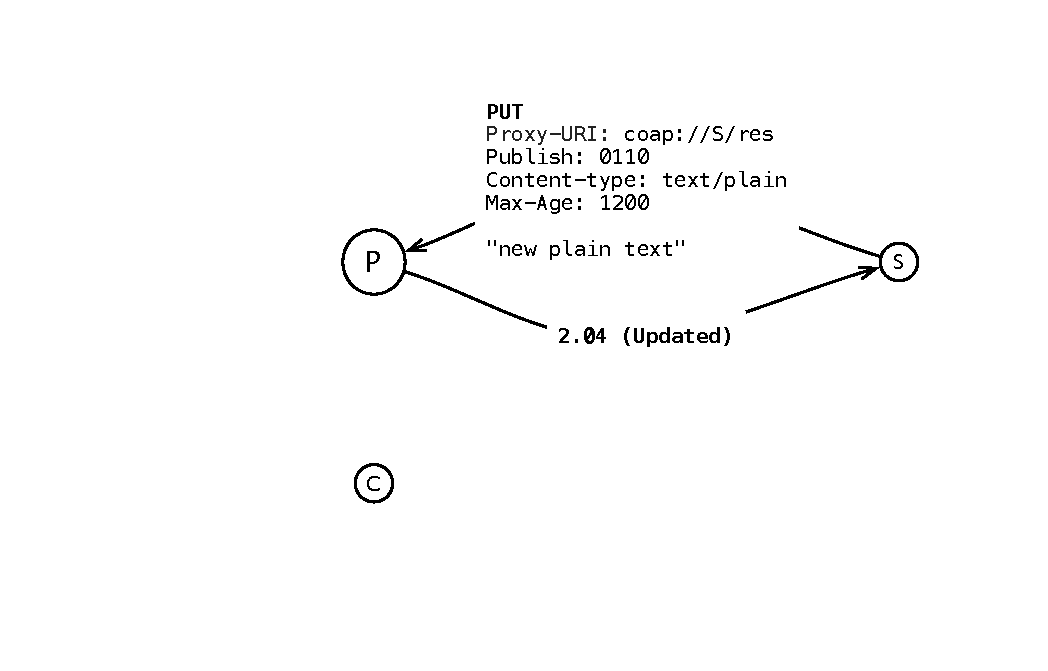
\includegraphics[width=\textwidth]{../../share/images/publish2.pdf}
 \end{center}
\end{frame}

%%
%% Publish (pic: retrieve published resource)
%%
\begin{frame}{(4) Act on updated resource}
 \begin{center}
  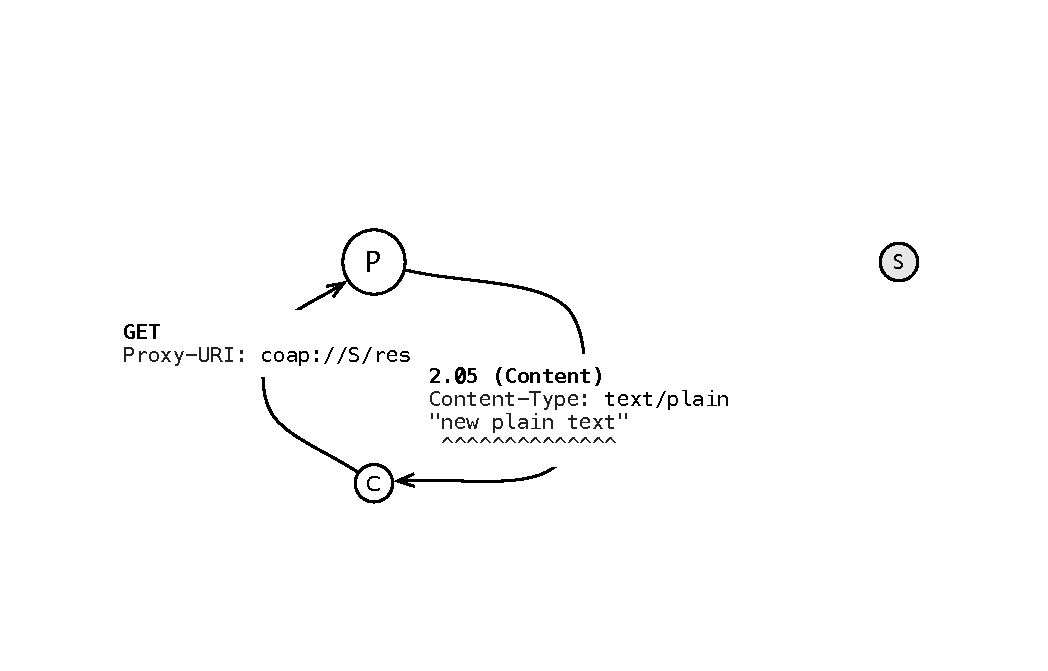
\includegraphics[width=\textwidth]{../../share/images/publish3.pdf}
 \end{center}
\end{frame}

%%
%% Publish (pic: remove delegation)
%%
\begin{frame}{(5) Remove delegation}
 \begin{center}
  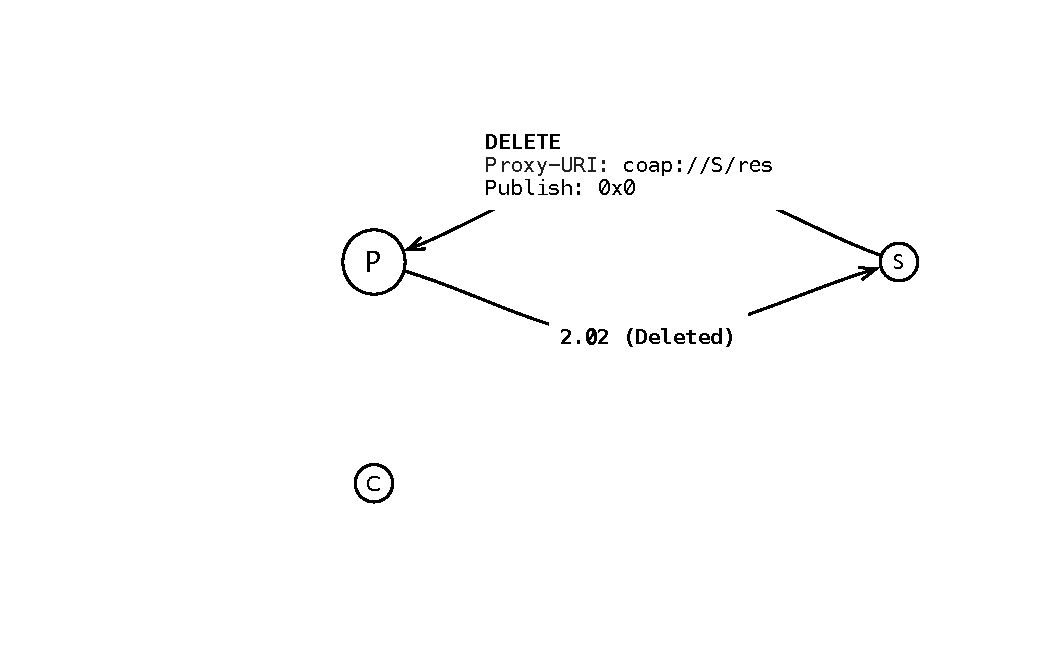
\includegraphics[width=\textwidth]{../../share/images/publish4.pdf}
 \end{center}
\end{frame}

%%
%% Publish (pic: removal)
%%
\begin{frame}{(6) Effect of delegation removal}
 \begin{center}
  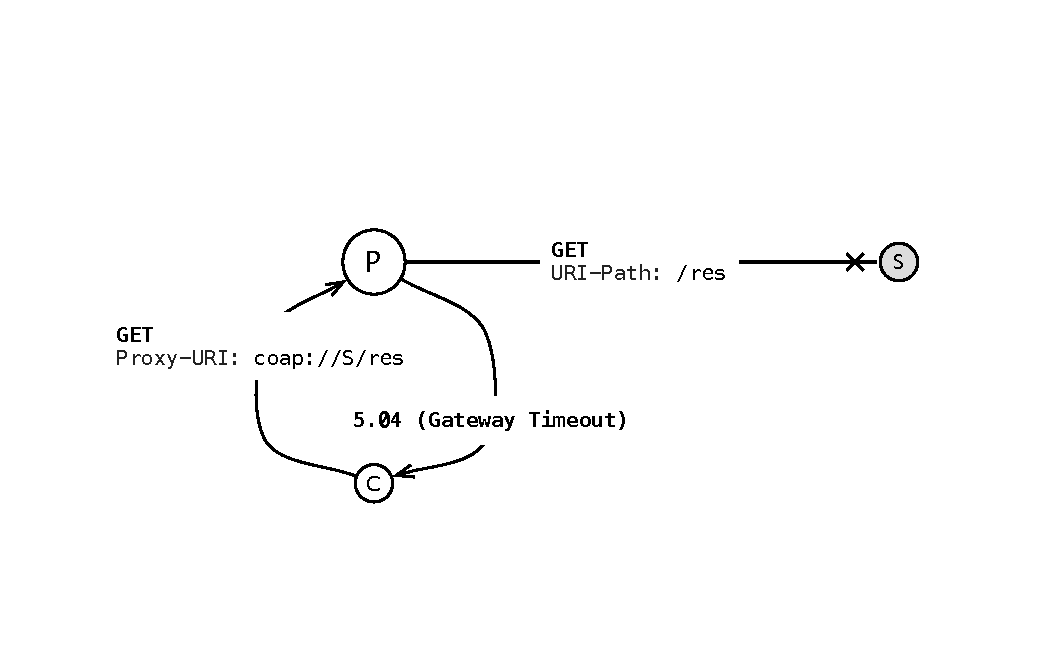
\includegraphics[width=\textwidth]{../../share/images/publish5.pdf}
 \end{center}
\end{frame}

%%
%% Pro
%%
\begin{frame}{Pro}

\begin{itemize}
 \item No URI proliferation %% the resource original URI is the only way to access the resource
 \item No soft state has to be maintained on sleepy client
 \item Explicit delegation lifetime
 \item Support writable resources
 \item Support Observe
\end{itemize}
\end{frame}

%%
%% Open issues
%%
\begin{frame}{Open issues}

\begin{itemize}
 \item Need \emph{strong mutual authentication} to authorize the delegation (and subsequent ops -- i.e. updates and deletion) on the resource
 \item Need to be coerced to one only delegation relationship to ensure consistency
\end{itemize}

\end{frame}

%%
%% Monitor option 
%%
\begin{frame}{Monitor \hspace{5cm} {\tiny \texttt{draft-fossati-core-publish-monitor-options-01}}}

\begin{itemize}
 \item Allow Observe to work in presence of Sleepy nodes %% bootstrap + lost notifications
 \item Solve bootstrap issue in case {\scriptsize $wake(S_1) \cap wake(S_2) = \emptyset$}
\end{itemize}

\end{frame}

\end{document}
